% Created 2011-03-18 Fri 14:56
\documentclass[11pt,article,oneside]{memoir} 
%\input{vc} % vc package
\usepackage[minted]{org-preamble-xelatex}
\usepackage{graphicx}
\usepackage{longtable}
\usepackage{float}
\providecommand{\alert}[1]{\textbf{#1}}

\title{Choosing Your Workflow Applications}
\author{Kieran Healy \\ \emph{Duke University}}
\date{}

\begin{document}

\maketitle


\thispagestyle{kjhgit}

\begin{abstract}
  As a beginning graduate student in the social sciences, what sort of
  software should you use to do your work? More importantly, what
  principles should guide your choices? This article offers some
  answers. The short version is: write using a good text editor (there
  are several to choose from); analyze quantitative data with R or
  Stata; minimize errors by storing your work in a simple format
  (plain text is best) and documenting it properly. Keep your projects
  in a version control system. Back everything up regularly and
  automatically. Don't get bogged down by gadgets, utilities or other
  accoutrements: they are there to help you do your work, but often
  waste your time by tempting you to tweak, update and generally futz
  with them. To help you get started, I provide a short discussion of
  the \href{http://kjhealy.github.com/emacs-starter-kit/}{Emacs
    Starter Kit for the Social Sciences}, a drop-in set of useful
  defaults designed to help you get started using Emacs (a powerful,
  free text-editor) for data analysis and writing.
\end{abstract}

\section*{Introduction}
\label{sec-1}

You can do productive, maintainable and reproducible work with all
kinds of different software set-ups.\symbolfootnote[0]{Email:
  \url{kjhealy@soc.duke.edu}. I thank Jake Bowers for helpful
  comments.} This is the main reason I don't go around encouraging
everyone to convert to the applications I use. (My rule is that I
don't try to persuade anyone to switch if I can't commit to offering
them technical support during and after their move.) So this
discussion is not geared toward convincing you there is One True Way
to organize things. I do think, however, that if you're in the early
phase of your career as a graduate student in, say, Sociology, or
Economics, or Political Science, you should give some thought to how
you're going to organize and manage your work.\footnote{This may also
  be true if you are about to move from being a graduate student to
  starting as a faculty member, though perhaps the rationale is less
  compelling given the costs. } This is so for two reasons. First, the
transition to graduate school is a good time to make changes. Early
on, there's less inertia and cost associated with switching things
around than there will be later. Second, in the social sciences, text
and data management skills are usually not taught to students
explicitly. This means that you may end up adopting the practices of
your advisor or mentor, continue to use what you are taught in your
methods classes, or just copy whatever your peers are doing. Following
these paths may lead you to an arrangement that you will be happy
with. But maybe not. It's worth looking at the options.

Two remarks at the outset. First, because this discussion is aimed at
beginning students, some readers may find much with which they are
already familiar. Even so, some sections may still be of interest, as
I have tried to keep the software references quite current. Second,
although in what follows I advocate you take a look at several
applications in particular, it's not really about the gadgets or
utilities. The Zen of Organization is Not to be Found in Fancy
Software. Nor shall the true path of Getting Things Done be revealed
to you through the purchase of a nice
\href{http://www.moleskineus.com/}{Moleskine Notebook}. Instead, it
lies within---unfortunately.

\section*{Just Make Sure You Know What You Did}
\label{sec-2}
For any kind of formal data analysis that leads to a scholarly paper,
however you do it, there are some basic principles to adhere
to. Perhaps the most important thing is to do your work in a way that
leaves a coherent record of your actions. Instead of doing a bit of
statistical work and then just keeping the resulting table of results
or graphic that you produced, for instance, write down what you did as
a documented piece of code. Rather than figuring out but not recording
a solution to a problem you might have again, write down the answer as
an explicit procedure. Instead of copying out some archival material
without much context, file the source properly, or at least a precise
reference to it.

Why should you bother to do any of this? Because when you inevitably
return to your table or figure or quotation nine months down the line,
your future self will have been saved hours spent wondering what it
was you thought you were doing and where you got that result from.

A second principle is that a document, file or folder should always be
able to tell you what it is. Beyond making your work reproducible, you
will also need some method for organizing and documenting your draft
papers, code, field notes, datasets, output files or whatever it is
you're working with. In a world of easily searchable files, this may
mean little more than keeping your work in plain text and giving it a
descriptive name. It should generally \emph{not} mean investing time
creating some elaborate classification scheme or catalog that becomes
an end in itself to maintain.

A third principle is that repetitive and error-prone processes should
be automated if possible. (Software developers call this ``DRY'', or
\href{http://en.wikipedia.org/wiki/Don't_repeat_yourself}{Don't Repeat
  Yourself.}) This makes it easier to check for and correct
mistakes. Rather than copying and pasting code over and over to do
basically the same thing to different parts of your data, write a
general function that can be called whenever it's needed. Instead of
retyping and reformatting the bibliography for each of your papers as
you send it out to a journal, use software that can manage this for
you automatically.

There are many ways of implementing these principles. You could use
Microsoft Word, Endnote and SPSS. Or Textpad and Stata. Or a pile of
legal pads, a calculator, a pair of scissors and a box of file
folders. Still, software applications are not all created equal, and
some make it easier than others to do the Right Thing. For instance,
it is \emph{possible} to produce well-structured, easily-maintainable
documents using Microsoft Word. But you have to use its styling and
outlining features strictly and responsibly, and most people don't
bother. You can maintain reproducible analyses in SPSS, but the
application isn't set up to do this automatically or efficiently, nor
does its design encourage good habits. So, it is probably a good idea
to invest some time learning about the alternatives. Many of them are
free to use or try out, and you are at a point in your career where
you can afford to play with different setups without too much trouble.

\section*{What Sort of Computer Should You Use?}
\label{sec-3}
The earliest choice you will face is buying your computer and deciding
what operating system to run on it. The leading candidates are
Microsoft Windows, Apple's Mac OS X, and some distribution of
Linux. Each of these platforms has gone some of the way --- in some
cases a long way --- toward remedying the main defects stereotypically
associated with it. I would characterize the present state of things
this way:


\begin{itemize}
\item Windows dominates the market. Because of this, far more viruses and
  malware target Windows than any other OS. Long-standing design and
  usability problems have been somewhat ameliorated in recent
  years. The previous major version, Windows Vista, was not very
  popular, though its main problems were not primarily related to
  security. Its successor, Windows 7, is generally accepted to be a
  solid improvement.
\item Mac OS X runs only on computers made by Apple (the existence of
  ``hackintoshes'' notwithstanding). Unlike in the past, Apple
  computers today have the same basic hardware as computers that run
  Windows. This has two consequences for those considering Mac OS
  X. First, one can now make direct price comparisons between Apple
  computers and PC alternatives (such as Dells, Lenovos, etc). In
  general, the more similarly kitted-out a PC is to an Apple machine,
  the more the price difference between the two goes
  away.\footnote{Comparisons should still take account of remaining
    differences in hardware design quality, and of course the OS
    itself. } However, Apple does not compete at all price-points in
  the market, so it will always be possible to configure a cheaper PC
  (with fewer features) than one Apple sells. For the same reason, it
  is also easier to find a PC configuration precisely tailored to some
  particular set of needs or preferences (e.g., with a better display
  but without some other feature or other) than may be available from
  Apple.

  Second, because Apple now runs Intel-based hardware, installing and
  running Windows is easy, and even catered to by Mac OS's Boot Camp
  utility. Beyond installing OS X and Windows side-by-side,
  third-party virtualization software is available (for about \$80
  from \href{http://www.vmware.com/products/fusion/}{VMWare} or
  \href{http://www.parallels.com/}{Parallels}, or free from
  \href{http://www.virtualbox.org/}{VirtualBox}) that allows you to
  run Windows or Linux seamlessly within OS X. Thus, Apple hardware is
  the only setup where you can easily try out each of the main desktop
  operating systems.
\item Linux is stable, secure, and free. User-oriented distributions
  such as \href{http://www.ubuntu.com/}{Ubuntu} are much
  better-integrated and well-organized than in the past. The user
  environment is friendlier now. Installing, upgrading and updating
  software --- a key point of frustration and time-wasting in older
  Linux distributions --- is also much better than it used to be, as
  Linux's package-management systems have matured. It remains true
  that Linux users are much more likely to be forced at some point to
  learn more than they might want to about the guts of their operating
  system.
\end{itemize}

These days, I use Mac OS X, and the discussion here reflects that
choice to some extent. But the other two options are also perfectly
viable alternatives, and most of the applications I will discuss are
freely available for all of these operating systems.

The dissertation, book, or articles you write will generally consist
of the main text, the results of data analysis (perhaps presented in
tables or figures) and the scholarly apparatus of notes and
references. Thus, as you put a paper or an entire dissertation
together you will want to be able to easily \textbf{edit text},
\textbf{analyze data} and \textbf{minimize error}. In the next section
I describe some applications and tools designed to let you do this
easily. They fit together well (by design) and are all freely
available for Windows, Linux and Mac OS X. They are not perfect, by
any means --- in fact, some of them can be awkward to learn. But
graduate-level research and writing can also be awkward to
learn. Specialized tasks need specialized tools and, unfortunately,
although they are very good at what they do, these tools don't always
go out of their way to be friendly.
\section*{Edit Text}
\label{sec-4}

If you are going to be doing quantitative analysis of any kind then
you should write using a good text editor. The same can be said, I'd
argue, for working with any highly structured document subject to a
lot of revision, such as a scholarly paper. Text editors are different
from word processors. Unlike applications such as Microsoft Word, text
editors generally don't make a big effort to make what you write look
like as though it is being written on a printed page.\footnote{For
  further argument about the advantages of text-editors over word
  processors see Allin Cottrell's polemic,
  ``\href{http://www.ecn.wfu.edu/~cottrell/wp.html}{Word Processors:
    Stupid and Inefficient}.'' } Instead, they focus on working with
text efficiently and assisting you with visualizing the logical
structure of what you're writing. If you are writing code to do some
statistical analysis, for instance, then at a minimum a good editor
will highlight keywords and operators in a way that makes the code
more readable. Typically, it will also passively signal to you when
you've done something wrong syntactically (such as forget a closing
brace or semicolon or quotation mark), and
\href{http://en.wiktionary.org/wiki/automagical}{automagically} indent
or tidy up your code as you write it. If you are writing a scholarly
paper or a dissertation, a good text editor can make it easier to
maintain control over the structure of your document, and help ensure
that cross-references and other paraphernalia are correct. Just as the
actual numbers are crunched by your stats program --- not your text
editor --- the typesetting of your paper is handled by a specialized
application, too. Perhaps more importantly, a text editor
\emph{manipulates plain text} as opposed to binary file formats like
\texttt{.doc} or \texttt{.pdf}, and plain text is the easiest format
to manage, control, back up, and come back to later with some other
application.

\textbf{Emacs} is a text editor, in the same way the blue whale is a
mammal. Emacs is very powerful, and can become almost a complete
working environment in itself, should you so wish. (I don't really
recommend it.) Combining Emacs with some other applications and
add-ons (described below) allows you to manage writing and
data-analysis effectively. The
\href{http://www.gnu.org/software/emacs/}{Emacs Homepage} has links to
Windows and Linux versions. The two most easily available versions on
the Mac are \href{http://emacsformacosx.com/}{GNU Emacs} itself and
\href{http://aquamacs.org/}{Aquamacs}. The former is the ``purest''
version of Emacs and does not implement many Mac conventions out of
the box. The latter makes an effort to integrate Emacs with the Mac
OS. For Windows users who would like to use Emacs, the developers
maintain an
\href{http://www.gnu.org/software/emacs/windows/faq.html}{extensive
  FAQ} including information on where to download a copy and how to
install it.

While very powerful and flexible, Emacs is not particularly easy to
learn. Indeed, to many first-time users (especially those used to
standard applications on Windows or Mac OS) its conventions seem
bizarre and byzantine. As applications go, Emacs is quite ancient: the
first version was written by Richard Stallman in the 1970s. Because it
evolved in a much earlier era of computing (before decent graphical
displays, for instance, and possibly also fire), it doesn't share many
of the conventions of modern applications.\footnote{One of the reasons that Emacs' keyboard shortcuts are so
strange is that they have their roots in a model of computer that laid
out its command and function keys differently from modern
keyboards. It's that old. } Emacs offers many
opportunities to waste your time learning its particular conventions,
tweaking its settings, and generally customizing it. There are several
good alternatives on each major platform, and I discuss some of them
below.

At this point it's reasonable to ask why I am even mentioning it, let
alone recommending you try it. The answer is that, despite its
shortcomings, Emacs is nevertheless very, \emph{very} good at managing
the typesetting and statistics applications I'm about to discuss. It's
so good, in fact, that Emacs has recently become quite popular amongst
a set of software developers pretty much all of whom are much younger
than Emacs itself. The upshot is that there has been a run of good,
new resources available for learning it and optimizing it
easily. \href{http://peepcode.com/products/meet-emacs}{Meet Emacs}, a
screencast available for purchase from PeepCode, walks you through the
basics of the application. Emacs itself also has a built-in tutorial.

If text editors like Emacs are not concerned with formatting your
documents nicely, then how do you produce properly typeset papers? You
need a way to take the text you write and turn it into a presentable
printed (or PDF) page. This is what \textbf{\LaTeX{}} is for. \LaTeX{}
is a freely-available, professional-quality typesetting system. It
takes text marked up in a way that describes the structure and
formatting of the document (where the sections and subsections are,
for example, or whether text should be \textbf{in bold face} or
\emph{emphasized}) and typesets it properly. If you have ever edited
the HTML of a web page, you'll know the general idea of a markup
language. If you haven't, the easiest way to understand what I mean is
to look at a segment of \LaTeX{} markup. An example is shown in
Listing \ref{lst:latex}. You can get started with \LaTeX{} for Mac OS
X by downloading \href{http://tug.org/mactex/}{the MacTeX
  distribution}. On Windows,
\href{http://www.tug.org/protext/}{ProTeXt} and
\href{http://www.miktex.org/}{MiKTeX} are both widely-used. Linux
vendors have their own distributions, or you can install
\href{http://www.tug.org/texlive}{TeXLive} yourself.\footnote{For more
  about these distributions of \TeX{}, see the
  \href{http://www.latex-project.org/ftp.html}{\LaTeX{} project
    page}. The proliferation of ``-\TeX{}'' acronyms and names can be
  confusing to newcomers, as they may refer to a distribution of an
  entire \TeX{}/\LaTeX{} platform (as with MikTeX or MacTeX), or to a
  particular program or utility that comes with these distributions
  (such as BibTeX, for dealing with bibliographies), or to some bit of
  software that allows something else to work with or talk to the
  \TeX{} system. }

\begin{listing} 
\begin{minted}[bgcolor=bg,fontsize=\small]{tex}
\subsection{Edit Text} 
This is what \textbf{LaTeX} is for. LaTeX is a freely-available,
professional-quality typesetting system. It takes text marked up in
a way that describes the structure and formatting of the document
(where the sections and subsections are, for example, or whether
text should be \textbf{in bold face} or \emph{emphasized}) and
typesets it properly. If you have ever edited the HTML of a web
page, you'll know the general idea of a markup language. If you
haven't, the easiest way to understand what I mean is to look at a
segment of LaTeX markup. An example is shown in Listing
\ref{lst:latex}.
\end{minted}
\caption{Part of the \LaTeX\ source for an earlier version of this document.}
\label{lst:latex}
\end{listing}


\LaTeX{} works best with some tools that help you take full advantage
of it with a minimum of fuss. You can manage bibliographical
references in \LaTeX{} documents using \textbf{BibTeX}. It does the
same job as \textbf{\href{http://www.endnote.com/}{Endnote}}, the
commercial plug-in for managing references in Microsoft Word. BibTeX
comes with any standard \LaTeX{} installation. Whichever text editor
or word processor you use, you should strongly consider some kind of
reference-manager software for your bibliographies. It saves a
tremendous amount of time because you can easily switch between
bibliographical formats, and you don't have to worry whether every
item referenced in your dissertation or paper is contained in the
bibliography.\footnote{If you plan to use BibTeX to manage your
  references, take a look at
  \href{http://www.ctan.org/tex-archive/help/Catalogue/entries/biblatex.html}{BibLaTeX},
  a package by Philipp Lehman, together with
  \href{http://biblatex-biber.sourceforge.net/}{Biber}, a replacement
  for BibTeX. BibLaTeX and Biber are not yet officially stable, but
  they are very well-documented, in wide use, and will soon jointly
  replace BibTeX as the standard way to process bibliographies in
  \LaTeX{}. I recommend you use them instead of older configurations
  (such as BibTeX and the Natbib package) which you may come across in
  other introductory discussions. }

\textbf{\href{http://www.gnu.org/software/auctex/}{AUCTeX}} and
\textbf{RefTeX} are available for Emacs. These packages allow Emacs to
understand the ins-and-outs of typesetting \LaTeX{} documents,
color-coding the marked-up text to make it easier to read, providing
shortcuts to LaTeX's formatting commands, and helping you manage
references to Figures, Tables and bibliographic citations in the
text. These packages could also be listed under the ``Minimize Error''
section below, because they help ensure that your references and
bibliography will be complete and consistently formatted.\footnote{A
  note about fonts and \LaTeX{}. It used to be that getting \LaTeX{}
  to use anything but a relatively small set of fonts was a very
  tedious business. This is no longer the case. The
  \href{http://scripts.sil.org/cms/scripts/page.php?site_id=nrsi&id=xetex}{XeTeX}
  engine makes it trivially easy to use any Postscript, TrueType or
  OpenType font installed on your system. XeTeX was originally
  developed for use on the Mac, but is available now for Linux and
  Windows as well. If you want to use a variety of fonts with an
  absolute minimum of fuss, use the \texttt{xelatex} command to typset
  your documents instead of \texttt{pdflatex}. }

More information on Emacs and \LaTeX{} is readily available via Google,
and there are several excellent books available to help you get
started. \textcite{kopka03:_guide_latex} and
\textcite{mittlebach04:_latex_compan} are good resources for learning
\LaTeX{}.
     
\section*{Analyze Data and Present Results}
\label{sec-5}

You will probably be doing some --- perhaps a great deal --- of
quantitative data analysis. \textbf{R} is an environment for
statistical computing. It's exceptionally well-supported, continually
improving, and has a very active expert-user community who have
produced many add-on packages. R has the ability to produce
sophisticated and high-quality statistical graphics. The documentation
that comes with the software is complete, if somewhat terse, but there
are a large number of excellent reference and teaching texts that
illustrate its use. These include
\textcite{dalgaard02:_introd_statis_r,
  venables02:_moder_applied_statis_s_plus,
  maindonald03:_data_analy_graph_using_r,
  fox02:_r_s_plus_compan_applied_regres, frank01:_regres_model_strat},
and \textcite{gelmanhill07:data_analysis}. Although it is a
command-line tool at its core, it has a good graphical interface as
well. You can download it from \href{http://www.r-project.org/}{The R
  Project Homepage}.

R can be used directly within Emacs by way of a package called
\textbf{ESS} (for ``Emacs Speaks Statistics''). As shown in Figure
\ref{fig:ess}, it allows you to work with your code in one Emacs frame
and a live R session in another right beside it. Because everything is
inside Emacs, it is easy to do things like send a chunk of your code
over to R using a keystroke. This is a very efficient way of doing
interactive data analysis while building up code you can use again in
future.

\begin{figure}[htb]
\centering
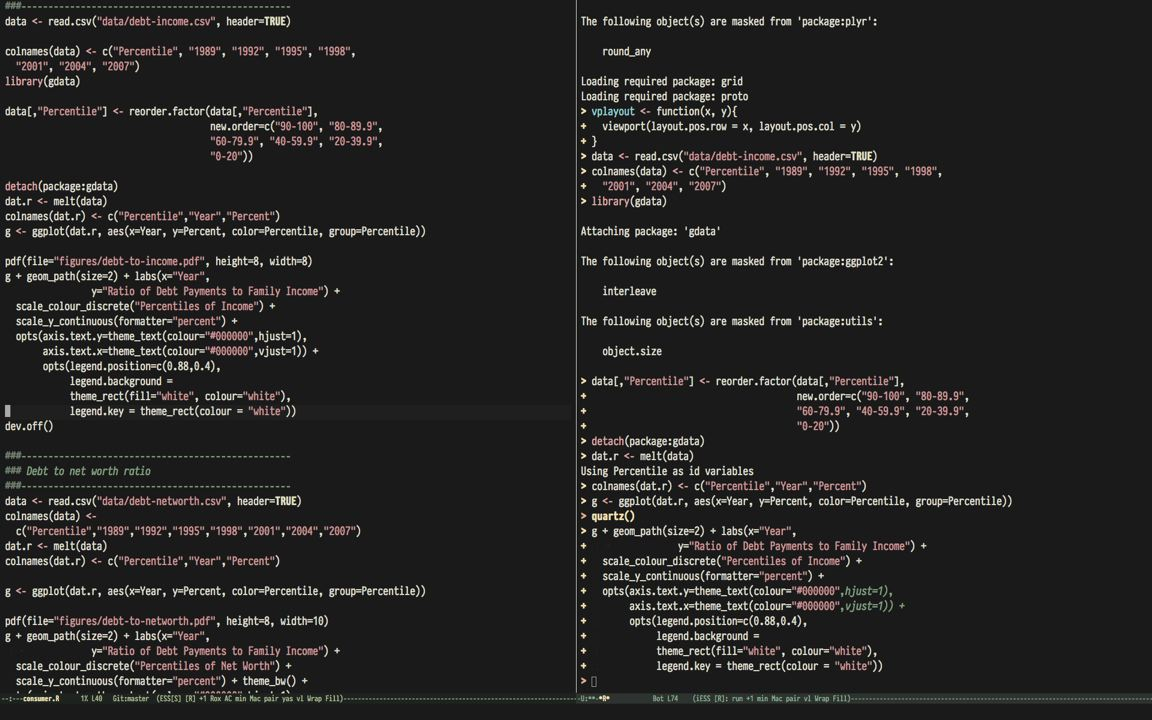
\includegraphics[width=5in]{figures/ess-r-emacs.png}
\caption{\label{fig:ess}An R session running inside Emacs using ESS. The R code file is on the left, and R itself is running on the right. You write in the left-hand pane and use a keyboard shortcut to send bits of code over to the right-hand pane, where they are executed by R.}
\end{figure}

You'll present your results in papers, but also in talks where you
will likely use some kind of presentation software. Microsoft's
PowerPoint is the most common application, but there are better
ones. If you wish, you can use \LaTeX{}, too, creating slides with the
\href{http://latex-beamer.sourceforge.net/}{Beamer document class} and
displaying them as full-screen PDFs. Alternatively, on Mac OS X
Apple's \href{http://www.apple.com/iwork/keynote/}{Keynote} is very
good. One benefit of using a Mac is that PDF is the operating system's
native display format, so PDF graphics created in R can simply be
dropped into Keynote without any compatibility problems. Microsoft's
PowerPoint is less friendly toward the clean integration of PDF files
in presentations.\footnote{The actual business of \emph{giving} talks
  based on your work is beyond the scope of this discussion. Suffice
  to say that there is plenty of good advice available via Google, and
  you should pay attention to it. }
                          
\section*{Minimize Error}
\label{sec-6}

We have already seen how the right set of tools can save you time by
automatically highlighting the syntax of your code, ensuring
everything you cite ends up in your bibliography, picking out mistakes
in your markup, and providing templates for commonly-used methods or
functions. Your time is saved twice over: you don't repeat yourself,
and you make fewer errors you'd otherwise have to fix. When it comes
to managing ongoing projects, minimizing error means addressing two
related problems. The first is to find ways to further reduce the
opportunity for errors to creep in without you noticing. This is
especially important when it comes to coding and analyzing data. The
second is to find a way to figure out, retrospectively, what it was
you did to generate a particular result. These problems are obviously
related, in that it's easy to make a retrospective assessment of
well-documented and error-free work. As a practical matter, we want a
convenient way to document work as we go, so that we can retrace our
steps in order to reproduce our results. We'll also want to be able to
smoothly recover from disaster when it befalls us.
 
Errors in data analysis often well up out of the gap that typically
exists between the procedure used to produce a figure or table in a
paper and the subsequent use of that output later. In the ordinary way
of doing things, you have the code for your data analysis in one file,
the output it produced in another, and the text of your paper in a
third file. You do the analysis, collect the output and copy the
relevant results into your paper, often manually reformatting them on
the way. Each of these transitions introduces the opportunity for
error. In particular, it is easy for a table of results to get
detached from the sequence of steps that produced it. Almost everyone
who has written a quantitative paper has been confronted with the
problem of reading an old draft containing results or figures that
need to be revisited or reproduced (as a result of peer-review, say)
but which lack any information about the circumstances of their
creation. Academic papers take a long time to get through the cycle of
writing, review, revision, and publication, even when you're working
hard the whole time. It is not uncommon to have to return to something
you did two years previously in order to answer some question or other
from a reviewer. You do not want to have to do everything over from
scratch in order to get the right answer. I am not exaggerating when I
say that, whatever the challenges of replicating the results of
someone else's quantitative analysis, after a fairly short period of
time authors themselves find it hard to replicate their \emph{own}
work. Computer Science people have a term of art for the inevitable
process of decay that overtakes a project simply in virtue of its
being left alone on the hard drive for six months or more: bit--rot.
\subsection*{Literate Programming with Sweave}
\label{sec-6_1}

A first step toward closing this gap is to use \textbf{Sweave} when
doing quantitative analysis in R. Sweave is a \emph{literate
  programming} framework designed to integrate the documentation of a
data analysis and its execution. You write the text of your paper (or,
more often, your report documenting a data analysis) as
normal. Whenever you want to run a model, produce a table or display a
figure, rather than paste in the results of your work from elsewhere,
you write down the R code that will produce the output you want. These
``chunks'' of code are distinguished from the regular text by a
special delimiter at their beginning and end. A small sample is shown
in Listing \ref{lst:codechunk}. The code chunk begins with the line
\texttt{<<load-data, echo=true>>=}. The character sequence
\texttt{<<>>=} is the marker for the beginning of a chunk:
\texttt{load-data} is just a label for the chunk and
\texttt{echo=true} is an option. The end of each chunk is marked by
the \texttt{@} symbol.

\begin{listing}
\begin{minted}[bgcolor=bg,fontsize=\small]{sweave}
\subsection{Some exploratory analysis}   
 In this section we do some exploratory analysis of the data. We begin
 by reading in the data file:
 
<<load-data, echo=true>>=
    ## load the data. 
    my.data <- read.csv("data/sampledata.csv",header=TRUE)
@  % The closing delimiter ends the code chunk.

 We should \emph{plot the data} to take a look at it:

<<plot-data, echo=true>>=
    ## make some plots.
    with(my.data, plot(x,y))
@

Maybe run some models, too.

<<ols-model echo=true>>=         
    ## OLS model
    out <- lm(y ~ x1 + x2,data=my.data)
    summary(out)
@ 
       
This concludes the exploratory analysis.
\end{minted}
\caption{\LaTeX\ and R code mixed together in an Sweave file.}
\label{lst:codechunk}
\end{listing}
 
When you're ready, you ``weave'' the file: you feed it to R, which
processes the code chunks, and spits out a finished version where the
code chunks have been replaced by their output. This is now a
well-formed \LaTeX{} file that you can then turn into a PDF document in
the normal way. Conversely, if you just want to extract the code
you've written from the surrounding text, then you ``tangle'' the file,
which results in an \texttt{.R} file. It's pretty straightforward in
practice. Sweave files can be edited in Emacs, as ESS understands
them.

The strength of this approach is that is makes it much easier to
document your work properly. There is just one file for both the data
analysis and the writeup. The output of the analysis is created on the
fly, and the code to do it is embedded in the paper. If you need to do
multiple but identical (or very similar) analyses of different bits of
data, Sweave can make generating consistent and reliable reports much
easier.\footnote{For some real-world case-studies of reproductions of
peer-reviewed studies using Sweave, and the errors uncovered as a
result, see \textcite{hothorn11:_case_studies_reprod}. }

A weakness of the Sweave model is that when you make changes, you have
to reprocess all of the code to reproduce the final \LaTeX{} file. If
your analysis is computationally intensive this can take a long
time. You can go a little ways toward working around this by designing
projects so that they are relatively modular, which is good practice
anyway. But for projects that are unavoidably large or computationally
intensive, the add-on package \texttt{cacheSweave}, available from the R
website, does a good job alleviating the problem.

\subsection*{Literate Programming with Org-mode}
\label{sec-6_2}

\textbf{\href{http://orgmode.org/}{Org-mode}} is an Emacs mode
originally designed to make it easier to take notes, make outlines and
manage to-do lists. Very much in the spirit of Emacs itself, its users
have extended it so that it is capable of all kinds of other things,
too, such as calendar management, time-tracking, and so on. One very
powerful extension to org-mode is
\href{http://orgmode.org/worg/org-contrib/babel/}{Org-Babel}, which is
a generalized literate-programming framework for org-mode
documents. It works like Sweave, except that instead of writing your
papers, reports, or documentation in \LaTeX{} and your code in R, you
write text in Org-mode's lightweight markup syntax and your code in
any one of a large number of supported languages. Org-mode has very
powerful export capabilities, so it can convert \texttt{.org} files to
\LaTeX{}, HTML, and many other formats quite easily. Examples of it in
use can be seen at the
\href{http://orgmode.org/worg/org-contrib/babel/intro.html}{Org-babel
  website}.  This article was written as a plain-text \texttt{.org}
file and the raw version is available for inspection
\href{https://github.com/kjhealy/workflow-paper}{as a repository on
  GitHub}. You can treat Org-Babel just as you would Sweave, or you
can take advantage of the fact that it's fully part of org-mode and
get all of the latter's functionality for free.

For example, Figure \ref{fig:org-babel-example} is generated on the
fly from source-code blocks included in the \texttt{.org} source for
this article. A piece of code can be executed, displayed, or both ---
as in the case of Listing \ref{lst:babel}. Then the figure can be
created directly. I don't show the code for this here, but you can
look in the \href{https://github.com/kjhealy/workflow-paper}{source
  file for this article} to see how it's done.

\begin{listing}
\begin{minted}[bgcolor=bg,fontsize=\small]{R}
library(ggplot2)
tea <- rnorm(100)
biscuits <- tea + rnorm(100,0,1.3)
\end{minted}


\caption{``Live'' code contained in this document.}
\label{lst:babel}
\end{listing}


\begin{figure}[htb]
\centering
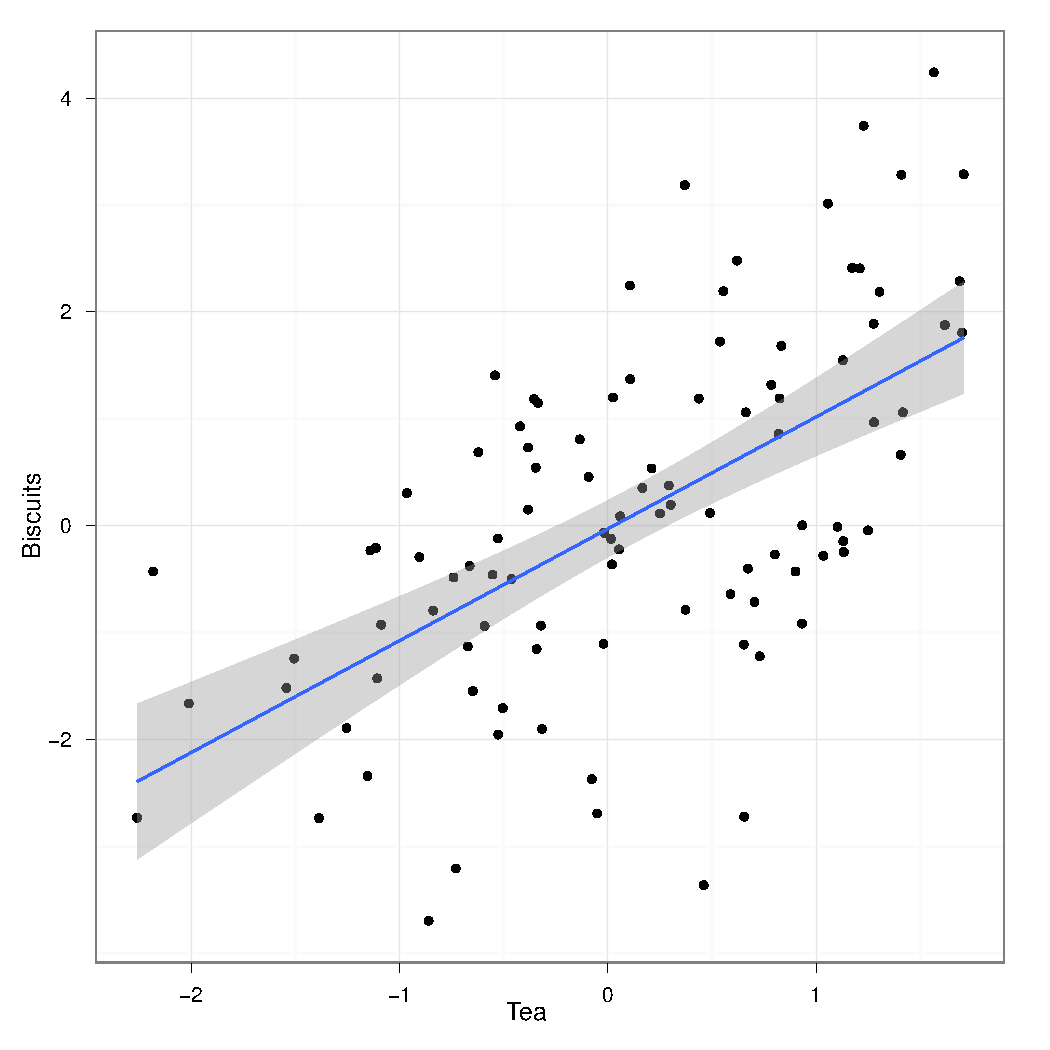
\includegraphics[width=4.5in]{figures/ggplot-example.pdf}
\caption{\label{fig:org-babel-example}A figure produced from code embedded in the source (\texttt{.org}) file for this article.}
\end{figure}

 
\subsection*{Use Revision Control}
\label{sec-6_3}

The task of documenting your work at the level of particular pieces of
code or edits to paragraphs in individual files can become more
involved over time, as projects grow and change. This can pose a
challenge to the Literate Programming model. Moreover, what if you are
not doing statistical analysis at all, but still want to keep track of
your work as it develops? The best thing to do is to institute some
kind of \textbf{version} \textbf{control} \textbf{system} to keep a
complete record of changes to a file, a folder, or a project. This can
be used in conjunction with or independently of a documentation method
like Sweave. A good version control system allows you to easily
``rewind the tape'' to earlier incarnations of your notes, drafts,
papers and code, and lets you keep track of what's current without
having to keep directories full of files with confusingly similar
names like \texttt{Paper-1.txt}, \texttt{Paper-2.txt},
\texttt{Paper-conferenceversion.txt}, and so on.

In the social sciences and humanities, you are most likely to have
come across the idea of version control by way of the ``Track
Changes'' feature in Microsoft Word, which lets you see the edits you
and your collaborators have made to a document. Think of true version
control as a way to keep track of whole projects (not just individual
documents) in a much better-organized, comprehensive, and transparent
fashion. Modern version control systems such as
\href{http://subversion.tigris.org/}{Subversion},
\href{http://www.selenic.com/mercurial/}{Mercurial} and
\href{http://git.or.cz/}{Git} can, if needed, manage very large
projects with many branches spread across multiple users. As such, you
have to get used to some new concepts related to tracking your files,
and then learn how your version control system implements these
concepts. Because of their power, these tools might seem like overkill
for individual users. (Again, though, many people find Word's ``Track
Changes'' feature indispensable once they begin using it.) But version
control systems can be used quite straightforwardly in a basic
fashion, and they increasingly come with front ends that can be easily
integrated with your text editor.\footnote{Emacs comes with support
  for a variety of VCS systems built in. There's also a very good
  add-on package, \href{http://philjackson.github.com/magit/}{Magit},
  devoted specifically to Git. } Moreover, you can meet these systems
half way. The excellent \href{https://www.getdropbox.com/}{DropBox},
for example, allows you to share files between different computers you
own, or with collaborators or general public. But it also
automatically version-controls the contents of these folders.

Revision control has significant benefits. A tool like Git or
Mercurial combines the virtues of version control with backups,
because every repository is a complete, self-contained,
cryptographically signed copy of the project. It puts you in the habit
of recording (or ``committing'') changes to a file or project as you
work on it, and (briefly) documenting those changes as you go. It
allows you to easily test out alternative lines of development by
branching a project. It allows collaborators to work on a project at
the same time without sending endless versions of the ``master'' copy
back and forth via email, and it provides powerful tools that allow
you to automatically merge or (when necessary) manually compare
changes that you or others have made. Perhaps most importantly, it
lets you revisit any stage of a project's development at will and
reconstruct what it was you were doing. This can be tremendously
useful whether you are writing code for a quantitative analysis,
managing field notes, or writing a paper.\footnote{Mercurial and Git
  are \emph{distributed} revision control systems (DVCSs) which can
  handle projects with many contributors and very complex,
  decentralized structures. Bryan O'Sullivan's
  \emph{\href{http://hgbook.red-bean.com/hgbook.pdf}{Distributed
      Version Control with Mercurial}} is a free, comprehensive guide
  to one of the main DVCS tools, but also provides a clear account of
  how modern version-control systems have developed, together with the
  main concepts behind them. For Git, I recommend starting
  \href{http://git-scm.com/}{at this site} and following the links to
  the documentation. } While you will probably not need to control
everything in this way (though some people do), I \emph{strongly}
suggest you consider managing at least the core set of text files that
make up your project (e.g., the code that does the analysis and
generates your tables and figures; the dataset itself; your notes and
working papers, the chapters of your dissertation, etc). As time goes
by you will generate a complete, annotated record of your actions that
is also a backup of your project at every stage of its
development. Services such as \href{http://www.github.com}{GitHub}
allow you to store public or (for a fee) private project repositories
and so can be a way to back up work offsite as well as a platform for
collaboration and documentation of your work.

\subsection*{You don't need backups until you really, really need them}
\label{sec-6_4}

Regardless of whether you choose to use a formal revision control
system, you should nevertheless have \emph{some} kind of systematic
method for keeping track of versions of your files. The task of
backing up and synchronizing your files is related to the question of
version control. Apple's Time Machine software, for example, backs up
and versions your files, allowing you to step back to particular
instances of the file you want. Other GUI-based file synchronization
tools, such as \href{http://www.getdropbox.com}{DropBox} and
\href{http://www.sugarsync.com/}{SugarSync}, are available across
various platforms.

Even if you have no need for a synchronization application, you will
still need to back up your work regularly. Because you are lazy and
prone to magical thinking, you will not do this responsibly by
yourself. This is why the most useful backup systems are the ones that
require a minimum amount of work to set up and, once organized, back
up everything automatically to an external (or remote) hard disk
without you having to remember to do anything. On Macs, Apple's
\textbf{Time Machine} software is built in to the operating system and
makes backups very easy. On Linux, you can use
\href{http://www.psychocats.net/ubuntu/backup}{rsync} for backups. It
is also worth looking into a secure, peer-to-peer, or offsite backup
service like \href{http://www.crashplan.com/}{Crashplan},
\href{https://spideroak.com/}{Spider Oak}, or
\href{http://www.backblaze.com/}{Backblaze}. Offsite backup means that
in the event (unlikely, but not unheard of) that your computer
\emph{and} your local backups are stolen or destroyed, you will still
have copies of your files.\footnote{I know of someone whose office
  building was hit by a tornado. She returned to find her files and
  computer sitting in a foot of water. You never know. } As Jamie
Zawinski \href{http://jwz.livejournal.com/801607.html}{has remarked},
when it comes to losing your data ``The universe tends toward maximum
irony. Don't push it.''

\section*{Pulling it Together: An Emacs Starter Kit for the Social Sciences}
\label{sec-7}

A step-by-step guide to downloading and installing every piece of
software I've mentioned so far is beyond the scope of this
discussion. But let's say you take the plunge and download Emacs, a
\TeX{} distribution, R, and maybe even Git. Now what? If you're going
to work in Emacs, there are a variety of tweaks and add-ons that are
very helpful but not set by default. To make things a little easier, I
maintain an \href{http://kjhealy.github.com/emacs-starter-kit/}{Emacs
  Starter Kit for the Social Sciences}. It's designed to smooth out
Emacs' rough edges by giving you a drop-in collection of default
settings, as well as automatically installing some important add-on
packages. It will, I hope, help you skirt the abyss of Setting Things
Up Forever. The
\href{http://github.com/technomancy/emacs-starter-kit/tree/master}{original
  version} of the kit was written by Phil Hagelberg and was made to go
with the ``\href{http://peepcode.com/products/meet-emacs}{Meet
  Emacs}'' screencast mentioned above. It was aimed at software
developers in general.  Eric Schulte, one of the authors of Org-babel,
\href{https://github.com/eschulte/emacs-starter-kit}{modified and
  further extended} the
kit. \href{https://github.com/kjhealy/emacs-starter-kit}{My version}
adds support for AucTeX, ESS, and other bits and pieces mentioned
here. As you can see if you follow the links, the kit is stored on
GitHub and you are free to fork it and modify it to your own liking.

\section*{Do I Have to Use this Stuff?}
\label{sec-8}
\subsection*{Pros and Cons}
\label{sec-8_1}

Using Emacs, \LaTeX{} and R together has four main advantages. First,
these applications are all free. You can try them out without much in
the way of monetary expense. (Your time may be a different matter, but
although you don't believe me, you have more of that now than you will
later.) Second, they are all open-source projects and are all
available for Mac OS X, Linux and Windows. Portability is important,
as is the long-term viability of the platform you choose to work
with. If you change your computing system, your work can move with you
easily. Third, they deliberately implement ``best practices'' in their
default configurations. Writing documents in \LaTeX{} encourages you to
produce papers with a clear structure, and the output itself is of
very high quality aesthetically. Similarly, by default R implements
modern statistical methods in a way that discourages you from thinking
about statistics in terms of canned solutions to standard problems. It
also produces figures that accord with accepted standards of efficient
and effective information design. And fourth, the applications are
closely integrated. Everything (including version control systems) can
work inside Emacs, and all of them talk to or can take advantage of
the others. R can output \LaTeX{} tables, for instance, even if you don't
use Sweave.

None of these applications is perfect. They are powerful, but they can
be hard to learn. However, you don't have to start out using all of
them at once, or learn everything about them right away --- the only
thing you \emph{really} need to start doing immediately is keeping
good backups. There are a number of ways to try them out in whole or
in part. You could try \LaTeX{} first, using any editor. Or you could
try Emacs and \LaTeX{} together. You could begin using R and its
GUI.\footnote{If you already know Emacs, you should certainly try R
  using ESS instead of the R GUI, though. } Sweave or Org-babel can be
left till last, though I have found these increasingly useful since
I've started using them, and wish that all of my old project
directories had some documentation in one or other of these
formats. Revision control is more beneficial when implemented at the
beginning of projects, and best of all when committing changes to a
project becomes a habit of work. But it can be added at any time.

You are not condemned to use these applications forever, either. \LaTeX{}
and (especially) Org-mode documents can be converted into many other
formats. Your text files are editable in any other text
editor. Statistical code is by nature much less portable, but the
openness of R means that it is not likely to become obsolete or
inaccessible any time soon.

A disadvantage of these particular applications is that I'm in a
minority with respect to other people in my field. This is less and
less true in the case of R, but remains so for \LaTeX{}. (It also
varies across social science disciplines.) Most people use Microsoft
Word to write papers, and if you're collaborating with people (people
you can't boss around, I mean) this can be an issue. Similarly,
journals and presses in my field often do not accept material marked
up in \LaTeX{}, though again there are important
exceptions. Converting files to a format Word understands can be
tedious (although it is quite doable).\footnote{Getting from \LaTeX{}
  to Word is easiest via HTML. But if you really want to maximize the
  portability of your papers or especially your reading notes or
  memos, consider writing them in a modern lightweight markup
  format. Org-mode's native format is effectively one of these
  already, and it provides built-in support for export to many
  others. An org-mode file can also be exported easily to rich-text or
  HTML, and from there Word or Google Docs will open it. Other options
  for lightweight markup include
  \href{http://en.wikipedia.org/wiki/Markdown}{Markdown} or its close
  relation,
  \href{http://fletcherpenney.net/MultiMarkdown}{MultiMarkdown}. Documents
  written in these formats are easy to read in their plain-text form
  but can be simply and directly converted into HTML, Rich Text,
  \LaTeX{}, Word, or other formats. TextMate has good support for
  Markdown and MultiMarkdown, allowing you to do these conversions
  more or less automatically. John MacFarlane's
  \href{http://johnmacfarlane.net/pandoc/}{Pandoc} is a powerful tool
  that can read markdown and (subsets of) reStructuredText, HTML, Org,
  and \LaTeX{}; and it can write to MarkDown, reStructuredText, HTML,
  \LaTeX{}, ConTeXt, RTF, DocBook XML, groff man, and S5 HTML slide
  shows. Pandoc is terrifically useful and I recommend checking it
  out. Lightweight markup languages like Markdown and Textile have a
  harder time dealing with some of the requirements of scholarly
  writing, especially the machinery of bibliographies and
  citations. If they could handle this task elegantly they would be
  almost perfect, but in practice this would probably just turn them
  back into something much less lightweight. Even here, though, good
  progress is being made as Pandoc will soon include support for
  citations. } I find these difficulties are outweighed by the
day-to-day benefits of using these applications, on the one hand, and
their longer-term advantages of portability and simplicity, on the
other. Your mileage, as they say, may vary.

\subsection*{Some Alternatives}
\label{sec-8_2}

There are many other applications you might put at the center of your
workflow, depending on need, personal preference, willingness to pay
some money, or desire to work on a specific platform. For text
editing, especially, there is a plethora of choices. On the Mac,
quality editors include
\href{http://www.barebones.com/products/bbedit/index.shtml}{BBEdit}
(beloved of many web developers),
\href{http://smultron.sourceforge.net/}{Smultron}, and
\href{http://macromates.com/}{TextMate} (shown in Figure
\ref{fig:tm}). TextMate has strong support for \LaTeX{} and good
(meaning, ESS-like) support for R. Because it is a modern application
written specifically for the Mac it can take advantage of features of
OS X that Emacs cannot, and is much better integrated with the rest of
the operating system. It also has good support for many of the
ancillary applications discussed above, such as version control
systems.\footnote{Its next major version, TextMate 2, has been in
  development for a very long time and is awaited with a mixture of
  near-religious hope, chronic anxiety and deep frustration by users
  of the original. } On Linux, an alternative to Emacs is
\href{http://www.eng.hawaii.edu/Tutor/vi.html}{vi} or
\href{http://www.vim.org/}{Vim}, but there are many others. For
Windows there is \href{http://www.textpad.com/}{Textpad},
\href{http://www.winedt.com/}{WinEdt},
\href{http://www.ultraedit.com/}{UltraEdit}, and
\href{http://notepad-plus.sourceforge.net/uk/site.htm}{NotePad++}
amongst many others. Most of these applications have strong support
for \LaTeX{} and some also have good support for statistics
programming.

\begin{figure}[htb]
\centering
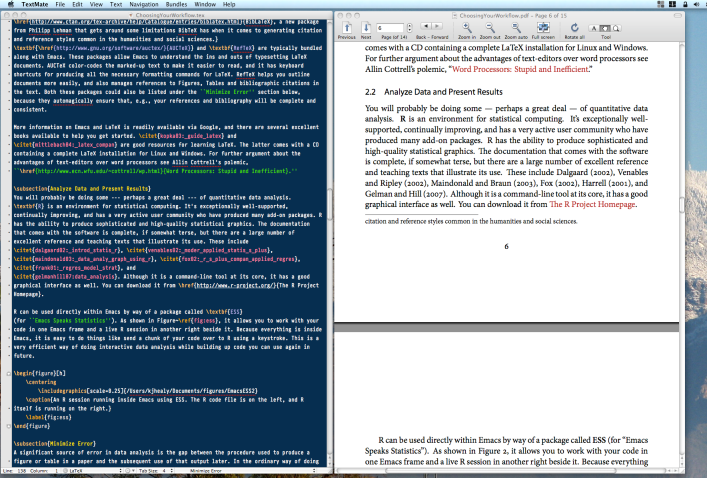
\includegraphics[width=5in]{figures/textmate.png}
\caption{\label{fig:tm}An earlier version of this document being edited in TextMate.}
\end{figure}

For statistical analysis in the social sciences, the main alternative
to R is \href{http://www.stata.com/}{Stata}. Stata is not free, but
like R it is versatile, powerful, extensible and available for all the
main computing platforms. It has a large body of user-contributed
software. In recent versions its graphics capabilities have improved a
great deal. ESS can run Stata inside Emacs in the same way as it can
do for R. Other editors can also be made to work with Stata: Jeremy
Freese provides an
\href{http://www.jeremyfreese.com/#other%20research}{UltraEdit syntax highlighting file for Stata}.  There is a \href{http://www.winedt.org/Config/modes/Stata.php}{Stata mode}
  for WinEdt. Friedrich Huebler has a
  \href{http://mysite.verizon.net/huebler/2005/20050310_Stata_editor.html}{guide
    for integrating Stata with programming editors}. Gabriel Rossman's
  blog \href{http://codeandculture.wordpress.com/tag/stata/}{Code and
    Culture} has many examples of using Stata in the day-to-day
  business of analyzing sociological data.

  Amongst social scientists, revision control is perhaps the least
  widely-used of the tools I have discussed. But I am convinced that
  it is the most important one over the long term. While tools like
  Git and Mercurial take a little getting used to both conceptually
  and in practice, the services they provide are extremely useful. It
  is already quite easy to use version control in conjunction with
  some of the text editors discussed above: Emacs and TextMate both
  have support for various DVCSs. On the Mac,
  \href{http://www.zennaware.com/cornerstone/}{CornerStone} and
  \href{http://www.versionsapp.com/}{Versions} are full-featured
  applications designed to make it easy to use Subversion. Taking a
  longer view, version control is likely to become more widely
  available through intermediary services or even as part of the basic
  functionality of operating systems.


\section*{A Broader Perspective}
\label{sec-9}

It would be nice if all you needed to do your work was a box software
of software tricks and shortcuts. But of course it's a bit more
complicated than that. In order to get to the point where you can
write a paper, you need to be organized enough to have read the right
literature, maybe collected some data, and most importantly asked an
interesting question in the first place. No amount of software is
going to solve those problems for you. Too much concern with the
details of your setup hinders your work. Indeed --- and I speak from
experience here --- this concern is itself a kind self-imposed
distraction that placates work-related anxiety in the short term while
storing up more of it for later.\footnote{See
  \href{http://inboxzero.com/}{Merlin Mann}, amongst others, for more
  on this point. } On the hardware side, there's the absurd
productivity counterpart to the hedonic treadmill, where for some
reason it's hard to get through the to-do list even though the café
you're at contains more computing power than was available to the
Pentagon in 1965. On the software side, the besetting vice of
productivity-enhancing software is the tendency to waste a lot of your
time installing, updating, and generally obsessing about your
productivity-enhancing software.\footnote{Mike Hall's brilliant
  ``\href{http://mph.puddingbowl.org/2010/02/org-mode-in-your-pocket-is-a-gnu-shaped-devil/}{Org-Mode
    in your Pocket is a GNU-Shaped Devil}'' makes this point very
  well. } Even more generally, efficient workflow habits are
themselves just a means to the end of completing the projects you are
really interested in, of making the things you want to make, of
finding the answers to the questions that brought you to graduate
school. The process of idea generation and project management can be
run well, too, and perhaps even the business of choosing what the
projects should be in the first place. But this is not the place ---
and I am not the person --- to be giving advice about that.

All of which is just to reiterate that it's the principles of workflow
management that are important. The software is just a means to an
end. One of the
\href{http://en.wikipedia.org/wiki/David_Kellogg_Lewis}{smartest, most
  productive people I've ever known} spent half of his career writing
on a typewriter and the other half on an
\href{http://www-03.ibm.com/ibm/history/exhibits/pc/pc_8.html}{IBM
  Displaywriter}. His backup solution for having hopelessly outdated
hardware was to keep a spare Displaywriter in a nearby closet, in case
the first one broke. It never did.

\printbibliography

\end{document}